\documentclass[11pt,a4paper]{article}

\usepackage[margin=2.2cm,top=2.5cm,bottom=2.5cm]{geometry}
\usepackage{amsmath,amssymb}
\usepackage{graphicx}
\usepackage[dvipsnames,svgnames,x11names]{xcolor}
\usepackage{tikz}
\usetikzlibrary{shapes,arrows.meta,positioning,calc,decorations.pathreplacing,shadows,fit}
\usepackage{booktabs}
\usepackage{tabularx}
\usepackage{fancyhdr}
\usepackage{hyperref}
\usepackage{enumitem}
\usepackage{tcolorbox}
\tcbuselibrary{skins,breakable}
\usepackage[T1]{fontenc}
\usepackage{lmodern}  % Vector fonts — eliminates bitmap rendering artifacts
\usepackage{titlesec}
\usepackage{float}
\usepackage{setspace}
\usepackage{parskip}
\usepackage{siunitx}

% ══════════════════════════════════════════════════════════════
% COLORS
% ══════════════════════════════════════════════════════════════
\definecolor{qnkpurple}{HTML}{7C3AED}
\definecolor{qnkblue}{HTML}{3B82F6}
\definecolor{qnkcyan}{HTML}{06B6D4}
\definecolor{qnkgreen}{HTML}{10B981}
\definecolor{qnkamber}{HTML}{F59E0B}
\definecolor{qnkred}{HTML}{EF4444}
\definecolor{qnkdark}{HTML}{0F172A}
\definecolor{qnkslate}{HTML}{334155}
\definecolor{qnkgold}{HTML}{D4AF37}
\definecolor{sectioncolor}{HTML}{5B21B6}
\definecolor{boxbg}{HTML}{F5F3FF}
\definecolor{keyboxbg}{HTML}{EFF6FF}
\definecolor{dbred}{HTML}{C0392B}
\definecolor{dborange}{HTML}{E67E22}
\definecolor{greenbox}{HTML}{F0FFF4}

% ══════════════════════════════════════════════════════════════
% STYLING
% ══════════════════════════════════════════════════════════════
\hypersetup{
    colorlinks=true,
    linkcolor=qnkpurple,
    urlcolor=qnkblue,
    citecolor=qnkpurple,
    pdfauthor={Quillon Foundation},
    pdftitle={Dragon Ball x Quillon -- FPGA Collaboration Proposal},
}

\pagestyle{fancy}
\fancyhf{}
\fancyhead[L]{\small\textcolor{qnkslate}{Dragon Ball Miner $\times$ Quillon --- FPGA Collaboration}}
\fancyhead[R]{\small\textcolor{qnkslate}{April 2026}}
\fancyfoot[C]{\small\textcolor{qnkslate}{\thepage}}
\renewcommand{\headrulewidth}{0.4pt}

\titleformat{\section}{\Large\bfseries\color{sectioncolor}}{}{0em}{}[\vspace{-0.5em}\textcolor{qnkpurple}{\rule{\textwidth}{1.5pt}}]
\titleformat{\subsection}{\large\bfseries\color{qnkslate}}{}{0em}{}

\newtcolorbox{keyinsight}[1][]{
    enhanced, colback=keyboxbg, colframe=qnkblue, boxrule=1pt, arc=4pt,
    left=10pt, right=10pt, top=8pt, bottom=8pt,
    fonttitle=\bfseries\color{qnkblue}, title={#1},
    shadow={1mm}{-1mm}{0mm}{black!15}
}
\newtcolorbox{highlight}[1][]{
    enhanced, colback=boxbg, colframe=qnkpurple, boxrule=1pt, arc=4pt,
    left=10pt, right=10pt, top=8pt, bottom=8pt,
    fonttitle=\bfseries\color{qnkpurple}, title={#1},
    shadow={1mm}{-1mm}{0mm}{black!15}
}
\newtcolorbox{greeninsight}[1][]{
    enhanced, colback=greenbox, colframe=qnkgreen, boxrule=1pt, arc=4pt,
    left=10pt, right=10pt, top=8pt, bottom=8pt,
    fonttitle=\bfseries\color{qnkgreen!80!black}, title={#1},
    shadow={1mm}{-1mm}{0mm}{black!15}
}

% ══════════════════════════════════════════════════════════════
% DOCUMENT
% ══════════════════════════════════════════════════════════════
\begin{document}

\begin{center}
{\Huge\bfseries\color{qnkpurple} Dragon Ball $\times$ Quillon}\\[6pt]
{\LARGE\color{qnkslate} FPGA Collaboration Proposal}\\[12pt]
{\large\color{qnkslate} Response to Chong's Technical Questions}\\[6pt]
{\normalsize\color{qnkslate} April 10, 2026 --- Quillon Foundation}\\[4pt]
\textcolor{qnkpurple}{\rule{0.6\textwidth}{2pt}}
\end{center}

\vspace{1em}

\begin{keyinsight}[Executive Summary]
Dragon Ball has proposed collaborating on the FPGA prototype phase of the QUG-V1 mining SoC. This document responds to Chong's specific technical questions about (1)~which algorithm the FPGA validates, (2)~whether Xilinx Artix-7 has sufficient resources, and (3)~how Dragon Ball can contribute to the FPGA phase. We propose a two-stage FPGA validation with Dragon Ball providing device selection expertise and FPGA manufacturing experience, while Quillon provides the complete RTL design and algorithm firmware.
\end{keyinsight}

% ══════════════════════════════════════════════════════════════
\section{Question 1: Which Algorithm Does the FPGA Validate?}
% ══════════════════════════════════════════════════════════════

\textbf{Answer: Both algorithms --- but in two stages within Phase~1.}

\subsection{Phase 1A: BLAKE3 Validation (Months 1--3)}

\begin{itemize}[leftmargin=1.5em]
    \item Validate the \textbf{Xcrypto BLAKE3 pipeline} (100 sequential hashes per nonce)
    \item Single-issue pipelined hash unit --- the simpler datapath
    \item \textbf{Purpose:} Prove the mining core works, validate hashrate/watt, test 16-core cluster interconnect
    \item This is the same class of problem as Dragon Ball's ALPH miner --- \textbf{familiar territory}
\end{itemize}

\subsection{Phase 1B: Genus-2 VDF Validation (Months 3--6)}

\begin{itemize}[leftmargin=1.5em]
    \item Validate the \textbf{Xlattice bignum accelerator} (256-bit modular arithmetic)
    \item Requires: Barrett reduction, modular multiplication, modular inversion (Fermat's method)
    \item \textbf{Purpose:} Prove the VDF acceleration works, measure doublings/sec/watt
    \item This is the \textbf{novel part} --- no one has done Genus-2 Jacobian hardware acceleration before
\end{itemize}

\begin{highlight}[Timeline Alignment]
Phase 1A can start \textbf{immediately}. The Genus-2 VDF algorithm is expected to activate on mainnet in Q3~2026, aligning perfectly with the Phase~1B FPGA validation timeline. Dragon Ball can evaluate the QUG-V1's performance on \emph{both} mining paths during the prototype phase.
\end{highlight}

\begin{center}
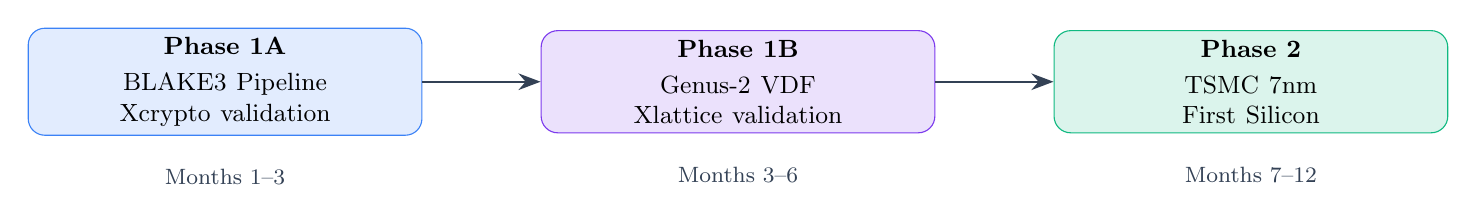
\begin{tikzpicture}[
    phase/.style={draw, rounded corners=6pt, minimum width=5cm, minimum height=1.2cm, text width=4.5cm, align=center, font=\small\bfseries},
    arrow/.style={-{Stealth[length=8pt]}, thick, color=qnkslate},
]
    \node[phase, fill=qnkblue!15, draw=qnkblue] (p1a) {Phase 1A\\[2pt]\normalfont\small BLAKE3 Pipeline\\Xcrypto validation};
    \node[phase, fill=qnkpurple!15, draw=qnkpurple, right=1.5cm of p1a] (p1b) {Phase 1B\\[2pt]\normalfont\small Genus-2 VDF\\Xlattice validation};
    \node[phase, fill=qnkgreen!15, draw=qnkgreen, right=1.5cm of p1b] (p2) {Phase 2\\[2pt]\normalfont\small TSMC 7nm\\First Silicon};

    \draw[arrow] (p1a) -- (p1b);
    \draw[arrow] (p1b) -- (p2);

    \node[below=0.3cm of p1a, font=\footnotesize\color{qnkslate}] {Months 1--3};
    \node[below=0.3cm of p1b, font=\footnotesize\color{qnkslate}] {Months 3--6};
    \node[below=0.3cm of p2, font=\footnotesize\color{qnkslate}] {Months 7--12};
\end{tikzpicture}
\end{center}

% ══════════════════════════════════════════════════════════════
\section{Question 2: Artix-7 Resource Assessment}
% ══════════════════════════════════════════════════════════════

\textbf{Chong's concern is correct.} The Xilinx Artix-7 (XC7A200T) is likely sufficient for Phase~1A but \textbf{insufficient for Phase~1B}.

\subsection{Artix-7 XC7A200T Resources}

\begin{center}
\begin{tabular}{@{}lrl@{}}
\toprule
\textbf{Resource} & \textbf{Available} & \textbf{Notes} \\
\midrule
Logic Cells & 215,360 & Adequate for single-core BLAKE3 \\
DSP48E1 Slices & 740 & \textcolor{dbred}{\textbf{Bottleneck for bignum}} \\
Block RAM (36Kb) & 365 & 13.14 Mb total \\
I/O Pins & 500 & Sufficient \\
\bottomrule
\end{tabular}
\end{center}

\subsection{Resource Estimates by Subsystem}

\begin{center}
\begin{tabular}{@{}lrrrl@{}}
\toprule
\textbf{Subsystem} & \textbf{LUTs} & \textbf{DSPs} & \textbf{BRAM} & \textbf{Fits Artix-7?} \\
\midrule
BLAKE3 Xcrypto pipeline (1 core) & $\sim$5K & 8 & 4 & \textcolor{qnkgreen}{\textbf{Yes}} \\
RISC-V core (RV32IMC) & $\sim$8K & 4 & 8 & \textcolor{qnkgreen}{\textbf{Yes}} \\
Bus + memory controller & $\sim$3K & 0 & 16 & \textcolor{qnkgreen}{\textbf{Yes}} \\
\textbf{Phase 1A total (1 mining core)} & \textbf{$\sim$16K} & \textbf{12} & \textbf{28} & \textcolor{qnkgreen}{\textbf{Yes (7\% util)}} \\
\midrule
256$\times$256 modular multiplier & $\sim$20K & 64--128 & 4 & \textcolor{qnkamber}{\textbf{Tight}} \\
Barrett reduction unit & $\sim$8K & 32 & 2 & \textcolor{qnkamber}{\textbf{Tight}} \\
8-butterfly parallel Xlattice & $\sim$80K & 512+ & 16 & \textcolor{dbred}{\textbf{No --- exceeds DSPs}} \\
\textbf{Phase 1B total (full SoC)} & \textbf{$\sim$150K} & \textbf{400+} & \textbf{64} & \textcolor{dbred}{\textbf{Needs larger FPGA}} \\
\bottomrule
\end{tabular}
\end{center}

\begin{keyinsight}[Dragon Ball's Insight is Correct]
The 8-butterfly parallel Xlattice unit requires 512+ DSP slices, which exceeds the Artix-7's 740 DSP budget when combined with the rest of the SoC. Dragon Ball's experience with the Xilinx 355T (likely Kintex-7 or Kintex UltraScale) for their previous FPGA prototypes is directly applicable here. We should select the FPGA device \textbf{together} based on Dragon Ball's manufacturing experience.
\end{keyinsight}

\subsection{Recommended FPGA Targets}

\begin{center}
\begin{tabular}{@{}llll@{}}
\toprule
\textbf{Validation Target} & \textbf{Recommended FPGA} & \textbf{Purpose} & \textbf{Est.\ Cost} \\
\midrule
BLAKE3 core only & Artix-7 200T & Phase 1A --- hash pipeline & \$500/board \\
Full SoC (1 core) & Kintex-7 355T or KU040 & Phase 1B --- complete mining core & \$2K--4K/board \\
Multi-core cluster (4 cores) & Virtex UltraScale+ & Optional --- interconnect validation & \$8K--15K/board \\
\bottomrule
\end{tabular}
\end{center}

\subsection{Direct Answer to Chong's Question}

\textbf{Phase 1A (BLAKE3 only):} Yes, Artix-7 A200T has sufficient resources. Our synthesis estimates show $\sim$16K LUTs, 12 DSPs, and 28 BRAM blocks --- just 7\% utilization. Artix-7 is viable and low cost for this phase.

\textbf{Phase 1B (Full SoC with Xlattice):} No, Artix-7 is insufficient. The 8-butterfly Xlattice unit alone needs 512+ DSPs, exceeding Artix-7's 740 budget when combined with the rest of the SoC. \textbf{Chong is correct} that a larger device is needed.

\subsection{Our Device Recommendation}

For Phase 1B, we recommend the \textbf{Xilinx Kintex-7 XC7K325T-2FFG900I}:

\begin{center}
\begin{tabular}{@{}lrrr@{}}
\toprule
\textbf{Resource} & \textbf{Kintex-7 325T} & \textbf{QUG-V1 Need} & \textbf{Margin} \\
\midrule
LUTs & 203,800 & $\sim$150K & 35\% headroom \\
DSP48E1 & 840 & $\sim$550 & 35\% headroom \\
Block RAM & 16.02 Mb & $\sim$10 Mb & 60\% headroom \\
Clock target & 200--300 MHz & 100 MHz (prototype) & Comfortable \\
\bottomrule
\end{tabular}
\end{center}

This part provides ample headroom, is in the same Kintex-7 family as Dragon Ball's existing 355T boards (toolchains and board designs may be reusable), and costs \$2K--4K per development board. We welcome Dragon Ball's confirmation or alternative suggestion based on your inventory.

% ══════════════════════════════════════════════════════════════
\section{Question 3: FPGA Collaboration Proposal}
% ══════════════════════════════════════════════════════════════

\textbf{Yes --- we warmly welcome Dragon Ball's involvement in the FPGA phase.} This strengthens both parties: Dragon Ball gains early insight into the algorithm, and Quillon benefits from Dragon Ball's FPGA manufacturing and verification expertise.

\subsection{Proposed Division of Work}

\begin{center}
\begin{tabular}{@{}p{7cm}p{7cm}@{}}
\toprule
\textbf{Quillon Provides} & \textbf{Dragon Ball Provides} \\
\midrule
Complete RTL design (Verilog/SystemVerilog) for QUG-V1 SoC & FPGA device selection expertise \\[4pt]
Mining algorithm firmware (BLAKE3 + Genus-2 VDF) & Board design and/or existing dev board access \\[4pt]
Testbench and verification suite & FPGA synthesis optimization \\[4pt]
Engineering support for ISA \& algorithm questions & Manufacturing cost estimates for 7nm (informed by FPGA results) \\[4pt]
Full NRE funding for Phase 1 (\$67.5K budgeted) & Engineering time (optional --- see cost models below) \\
\bottomrule
\end{tabular}
\end{center}

\subsection{Cost Sharing Models}

\begin{greeninsight}[Three Options --- Dragon Ball Chooses]
\begin{enumerate}[leftmargin=1.5em]
    \item \textbf{Pure OEM Model:} Quillon funds everything. Dragon Ball contributes engineering time only. Zero capital risk for Dragon Ball. Dragon Ball earns manufacturing margins on 7nm production.

    \item \textbf{Co-Development Model:} Dragon Ball provides FPGA boards and synthesis tools from existing inventory. Quillon provides RTL and firmware. Costs shared roughly 70/30 (Quillon/DB). Dragon Ball gets preferential manufacturing terms for 7nm.

    \item \textbf{Joint Venture Model:} Equal investment, equal revenue share. Dragon Ball co-owns the QUG-V1 design. Highest commitment, highest upside.
\end{enumerate}
We recommend starting with \textbf{Option 1 or 2} for the FPGA phase, then upgrading to Option 3 for 7nm if the partnership proves productive.
\end{greeninsight}

% ══════════════════════════════════════════════════════════════
\section{What We Need from Dragon Ball to Start}
% ══════════════════════════════════════════════════════════════

\begin{enumerate}[leftmargin=1.5em]
    \item \textbf{FPGA device recommendation:} Which Xilinx/AMD part do you recommend for validating the full SoC (Xlattice + Xcrypto + RISC-V core)? We are open to Kintex-7, Kintex UltraScale, or Virtex UltraScale+.

    \item \textbf{Existing infrastructure:} Do you have FPGA development boards from your ALPH/NEXA prototyping that we could target? Or should we design a new board?

    \item \textbf{Reference data:} Can you share your ALPH FPGA prototype specs? (Resource utilization, clock speed achieved, power consumption.) This helps us calibrate our estimates against real-world numbers.

    \item \textbf{Timeline estimate:} If we provide RTL by end of April, how quickly can your team synthesize, place-and-route, and test on an FPGA? (We expect 2--4 weeks for initial synthesis, 4--8 weeks for validation.)
\end{enumerate}

% ══════════════════════════════════════════════════════════════
\section{Next Steps}
% ══════════════════════════════════════════════════════════════

\begin{center}
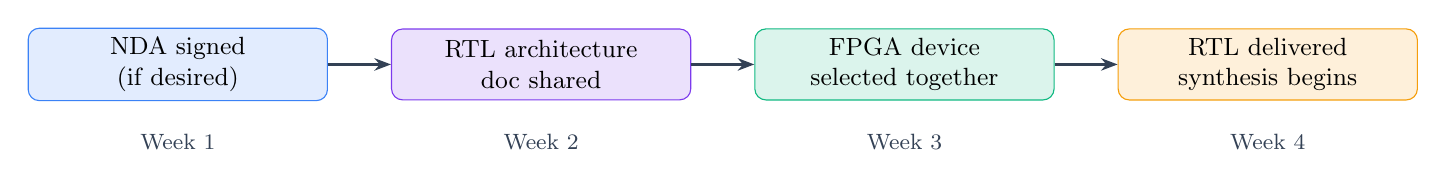
\begin{tikzpicture}[
    stepbox/.style={draw, rounded corners=4pt, minimum width=3.8cm, minimum height=0.9cm, text width=3.5cm, align=center, font=\small},
    arrow/.style={-{Stealth[length=6pt]}, thick, color=qnkslate},
]
    \node[stepbox, fill=qnkblue!15, draw=qnkblue] (s1) {NDA signed\\(if desired)};
    \node[stepbox, fill=qnkpurple!15, draw=qnkpurple, right=0.8cm of s1] (s2) {RTL architecture\\doc shared};
    \node[stepbox, fill=qnkgreen!15, draw=qnkgreen, right=0.8cm of s2] (s3) {FPGA device\\selected together};
    \node[stepbox, fill=qnkamber!15, draw=qnkamber, right=0.8cm of s3] (s4) {RTL delivered\\synthesis begins};

    \draw[arrow] (s1) -- (s2);
    \draw[arrow] (s2) -- (s3);
    \draw[arrow] (s3) -- (s4);

    \node[below=0.3cm of s1, font=\footnotesize\color{qnkslate}] {Week 1};
    \node[below=0.3cm of s2, font=\footnotesize\color{qnkslate}] {Week 2};
    \node[below=0.3cm of s3, font=\footnotesize\color{qnkslate}] {Week 3};
    \node[below=0.3cm of s4, font=\footnotesize\color{qnkslate}] {Week 4};
\end{tikzpicture}
\end{center}

\vspace{0.5em}

\begin{highlight}[Immediate Action]
If Chong is interested, we can share the RTL architecture document (block diagram, ISA encoding, memory map, bus protocol) this week. This is non-confidential technical specification --- not trade secrets. We can sign a mutual NDA first if Dragon Ball prefers.
\end{highlight}

% ══════════════════════════════════════════════════════════════
\section{Technical Reference: QUG-V1 Architecture Summary}
% ══════════════════════════════════════════════════════════════

For convenience, here is the QUG-V1 SoC architecture relevant to FPGA prototyping:

\begin{center}
\begin{tabular}{@{}lp{10cm}@{}}
\toprule
\textbf{Component} & \textbf{Description} \\
\midrule
CPU cores & 16$\times$ RISC-V RV32IMC (8 mining + 2 PQ-crypto + 4 network + 2 management) \\
Xcrypto extension & Opcode space custom-0 (0x0B). Pipelined BLAKE3 --- 9 cycles/hash at 1.5~GHz \\
Xlattice extension & Opcode space custom-1 (0x2B). 256-bit parallel modular arithmetic: \texttt{poly.mul}, \texttt{poly.reduce}, \texttt{ntt.fwd/inv}, \texttt{poly.add} \\
Memory & 2~MB shared SRAM + DDR4 controller (for full-node blockchain storage) \\
Interconnect & Crossbar NoC, 128-bit data bus, split transaction \\
I/O & PCIe Gen3 x4, GbE MAC, USB-C (management + firmware update) \\
Target process & TSMC N7 (Phase 2) $\to$ TSMC N5 (Phase 3) \\
Power & 9.5~W (N5 target), 12~W (N7 target) \\
\bottomrule
\end{tabular}
\end{center}

\vspace{1em}

\begin{center}
\textcolor{qnkslate}{\rule{0.4\textwidth}{0.5pt}}\\[6pt]
{\small\color{qnkslate} Full technical details available in:}\\[4pt]
{\small\color{qnkblue} \textit{QUG-V1 Pocket Supercomputer Whitepaper} (March 2026)}\\
{\small\color{qnkblue} \textit{Genus-2 Jacobian VDF Mining Whitepaper} (March 2026)}\\
{\small\color{qnkblue} \textit{Dragon Ball $\times$ Quillon Response v2} (April 2026)}
\end{center}

% ══════════════════════════════════════════════════════════════
\section{Why Dragon Ball Specifically}
% ══════════════════════════════════════════════════════════════

This is not a generic manufacturing RFP. Dragon Ball is uniquely positioned for this partnership:

\begin{itemize}[leftmargin=1.5em]
    \item \textbf{Proven TSMC 5nm/7nm access:} Dragon Ball already manufactures KAS and ALPH miners on advanced nodes. No other potential partner has this relationship already established.
    \item \textbf{Thermal engineering solved:} Dragon Ball designs ASICs at 3,000W. The QUG-V1's 9.5W is trivial by comparison --- zero thermal risk.
    \item \textbf{Mining distribution channels:} Dragon Ball already sells to the exact customer base that will buy QUG-V1 hardware. Immediate go-to-market.
    \item \textbf{FPGA prototyping infrastructure:} Dragon Ball's existing 355T boards and EDA toolchains can be reused, saving months.
\end{itemize}

No generic ODM (Flex, Jabil, Foxconn) can match this combination of silicon access, mining domain expertise, and distribution.

% ══════════════════════════════════════════════════════════════
\section{The Dual-Proof Advantage}
% ══════════════════════════════════════════════════════════════

Since the original proposal, Quillon has developed a \textbf{Dual-Proof mining system} that fundamentally changes the hardware landscape. The QUG-V1 is now the \emph{only} hardware that can mine both proof types efficiently.

\begin{center}
\begin{tabular}{@{}lccc@{}}
\toprule
\textbf{Hardware} & \textbf{BLAKE3 Path} & \textbf{Genus-2 VDF Path} & \textbf{Full Node} \\
\midrule
GPU (RTX 4090) & \textcolor{qnkgreen}{Efficient} & \textcolor{dbred}{Impossible (sequential)} & \textcolor{dbred}{No} \\
High-end CPU (i9-14900K) & \textcolor{dborange}{Moderate} & \textcolor{qnkgreen}{Moderate} & \textcolor{qnkgreen}{Yes (software)} \\
Raspberry Pi 5 & \textcolor{dbred}{Slow} & \textcolor{dbred}{Very slow} & \textcolor{qnkgreen}{Yes} \\
Traditional ASIC & \textcolor{qnkgreen}{Dominant} & \textcolor{dbred}{Cannot adapt} & \textcolor{dbred}{No} \\
\textbf{QUG-V1 (Quillon)} & \textcolor{qnkgreen}{\textbf{163$\times$ GPU}} & \textcolor{qnkgreen}{\textbf{$\sim$60$\times$ CPU efficiency}} & \textcolor{qnkgreen}{\textbf{Yes (hardware)}} \\
\bottomrule
\end{tabular}
\end{center}

\begin{highlight}[The Moat]
GPUs cannot mine the Genus-2 VDF path (inherently sequential). Traditional ASICs cannot adapt to algorithm changes (fixed-function silicon). CPUs can mine both paths but inefficiently. Only the QUG-V1 --- with \emph{both} Xcrypto and Xlattice on the same die --- dominates both mining paths while running a full node. This creates a \textbf{captive hardware market} with no substitutes.
\end{highlight}

\subsection{Genus-2 VDF Performance Projections}

\begin{center}
\begin{tabular}{@{}lrrr@{}}
\toprule
\textbf{Platform} & \textbf{Doublings/sec} & \textbf{Power} & \textbf{Efficiency (d/s/W)} \\
\midrule
x86 CPU (i9 @ 5 GHz) & $\sim$200 & 15W & 13.3 \\
ARM CPU (Cortex-A76 @ 2.4 GHz) & $\sim$80 & 3W & 26.7 \\
GPU (RTX 4090, 1 core) & $\sim$150 & 450W & 0.33 \\
\textbf{QUG-V1 Xlattice core (projected)} & \textbf{$\sim$500--800} & \textbf{0.6W/core} & \textbf{833--1,333} \\
\bottomrule
\end{tabular}
\end{center}

\textit{Note: QUG-V1 projections are based on architectural simulation, not silicon measurement. FPGA validation in Q3~2026 will provide measured performance data.}

% ══════════════════════════════════════════════════════════════
\section{Strategic Value for Dragon Ball}
% ══════════════════════════════════════════════════════════════

Beyond manufacturing margin (\$15--21/unit), this partnership offers Dragon Ball strategic advantages:

\begin{enumerate}[leftmargin=1.5em]
    \item \textbf{Customer acquisition funnel:} Every QUG-V1 buyer at \$149 is a potential future Dragon Ball ASIC customer at \$3K--15K. The low entry price creates a massive new customer base.

    \item \textbf{RISC-V capability:} Dragon Ball currently designs fixed-function ASICs. This partnership builds programmable SoC competence --- reusable across future products.

    \item \textbf{Network effect upside:} Unlike ASICs that depreciate as difficulty increases, QUG-V1 cards maintain value because they run full nodes and can adapt to algorithm changes via firmware. Dragon Ball can optionally embed a 1\% developer fee in firmware for ongoing revenue.

    \item \textbf{Diversification:} If the traditional ASIC market contracts (as it does cyclically), Dragon Ball has a consumer hardware product line as a hedge.

    \item \textbf{First-mover advantage:} No competitor has a RISC-V mining SoC. Dragon Ball would be the exclusive manufacturer of a new product category.
\end{enumerate}

% ══════════════════════════════════════════════════════════════
\section{IP Framework}
% ══════════════════════════════════════════════════════════════

\begin{center}
\begin{tabular}{@{}lp{10cm}@{}}
\toprule
\textbf{Asset} & \textbf{Ownership} \\
\midrule
QUG-V1 RTL design (Verilog/SV) & Quillon Foundation --- perpetual ownership \\
Xcrypto / Xlattice ISA extensions & Quillon Foundation --- perpetual ownership \\
Mining firmware \& blockchain software & Quillon Foundation --- open-source (MIT license) \\
GDSII mask works (7nm/5nm) & Jointly held by funding party (negotiable per cost model) \\
PCB / enclosure design (DOCK) & Dragon Ball --- owns mechanical/PCB design \\
Manufacturing license & Dragon Ball receives perpetual, royalty-free license to manufacture QUG-V1 \textbf{exclusively for Quillon} \\
Exclusivity window & Dragon Ball is sole manufacturer for 24 months post-launch \\
Third-party manufacturing & Not permitted during exclusivity window without mutual consent \\
\bottomrule
\end{tabular}
\end{center}

\textit{These terms are proposed starting points. Final IP terms will be negotiated in a definitive agreement after FPGA validation.}

% ══════════════════════════════════════════════════════════════
\section{Timeline \& Risk Mitigation}
% ══════════════════════════════════════════════════════════════

\begin{center}
\begin{tabular}{@{}lllp{5.5cm}@{}}
\toprule
\textbf{Phase} & \textbf{Target} & \textbf{Worst Case} & \textbf{Mitigation} \\
\midrule
FPGA prototype & Q3 2026 & Q4 2026 & Start Phase 1A immediately; Dragon Ball's existing boards \\
7nm tape-out & Q1 2027 & Q2 2027 & Use mature N7 process (high yield); budget \$500K for respin \\
First silicon validation & Q2 2027 & Q3 2027 & Start firmware dev on FPGA in Q3 2026, not after silicon \\
Volume production & Q3 2027 & Q1 2028 & 7nm ships as revenue product even if 5nm is delayed \\
5nm upgrade & Q1 2028 & Q3 2028 & 5nm is funded by 7nm revenue; not gating \\
\bottomrule
\end{tabular}
\end{center}

\begin{keyinsight}[Key Risk: 7nm Respin]
If first 7nm silicon requires a respin, the timeline extends by $\sim$6 months and costs an additional \$500K--1M. This risk is mitigated by: (1)~thorough FPGA validation before tape-out, (2)~using mature TSMC N7 with high yield, and (3)~Dragon Ball's existing tape-out experience reducing integration errors.
\end{keyinsight}

% ══════════════════════════════════════════════════════════════
\section{Product Roadmap 2026--2030}
% ══════════════════════════════════════════════════════════════

\begin{center}
\begin{tabular}{@{}llp{8cm}@{}}
\toprule
\textbf{Year} & \textbf{Product} & \textbf{Description} \\
\midrule
2026 H2 & FPGA prototype & Validate Xcrypto + Xlattice on Dragon Ball's FPGA boards \\
2027 H1 & QUG-V1 (7nm) & First silicon. 10 MH/s @ 12W. Credit-card form factor. \\
2027 H2 & DOCK-8 / DOCK-16 & Desktop enclosures. 8--16 card slots. \$99--199 per dock. \\
2028 H1 & QUG-V1 (5nm shrink) & 17 MH/s @ 9.5W. Same package, drop-in upgrade. \\
2028 H2 & QUG-V2 & More cores, integrated Wi-Fi 7, lower power. DOCK-compatible. \\
2029+ & QUG-V3 & Next-gen architecture. Post-quantum integrated. 3nm target. \\
\bottomrule
\end{tabular}
\end{center}

This is a \textbf{platform, not a one-off product}. Dragon Ball becomes the exclusive manufacturer for an entire product family spanning 5+ years.

\vspace{1.5em}

\begin{center}
\textcolor{qnkpurple}{\rule{0.5\textwidth}{1.5pt}}\\[8pt]
{\small\textcolor{qnkslate}{CONFIDENTIAL --- Dragon Ball Miner Only}}\\[4pt]
{\small\textcolor{qnkslate}{Quillon Foundation --- April 2026}}\\[4pt]
{\small\textcolor{qnkslate}{Contact: \href{mailto:overdrevetfedmetodologi@protonmail.com}{overdrevetfedmetodologi@protonmail.com}}}
\end{center}

\end{document}
